\documentclass[a4paper]{article}

\usepackage[utf8]{inputenc} % set input encoding (not needed with XeLaTeX)
\usepackage[spanish]{babel}

\usepackage[numbers]{natbib}         % bibliography style
\usepackage[colorlinks]{hyperref}    % better urls in bibliography

%%% SECTION TITLE APPEARANCE
\usepackage{sectsty}
\allsectionsfont{\sffamily\mdseries\upshape} % (See the fntguide.pdf for font help)
\usepackage{titling}
\newcommand{\subtitle}[1]{%
  \posttitle{%
    \par\end{center}
    \begin{center}\large#1\end{center}
    \vskip0.5em}%
}

%%% PAGE DIMENSIONS
\usepackage{geometry} % to change the page dimensions
\geometry{a4paper} % or letterpaper (US) or a5paper or....
% \geometry{margin=2in} % for example, change the margins to 2 inches all round
% \geometry{landscape} % set up the page for landscape
%   read geometry.pdf for detailed page layout information

\usepackage{graphicx} % support the \includegraphics command and options

%%% END Article customizations
%%% The "real" document content comes below...

\begin{document}

\title{Propuesta de Proyecto\\Problemas Especiales de Ingeniería en Computación}
\subtitle{Simulación de Piloteo de Drones con Realidad Aumentada Utilizando Sensores para Configuración del Ambiente Virtual}

\author{Aníbla Vásquez Clad\\
\texttt{aniavasq@espol.edu.ec}
\and Peter Arcentales\\
\texttt{arcental@espol.edu.ec}}

\maketitle

\section{Introducción y Justificación}
El uso de Drones o Vehículos Aéreos No Tripulados inicialmente con aplicaciones meramente militares se ha extendido a diversas áreas de la ciencia, este uso es muy frecuente en lugares donde una aeronave común tripulada difícilmente puede llegar, ya sea por factores ambientales o de espacio, o en circunstancias de alto riesgo. Los Drones pueden ser aplicados para tomar muestras, reconocimiento cartográfico e hidrológico, control y vigilancia y otras posibilidades no necesariamente militares.
El objetivo de este proyecto es crear una aplicación en la cual un usuario de un samrtphone o tablet pueda experimentar de forma virtual el uso de un Drone con la ayuda de realidad aumentada y sensores del dispositivo como GPS y acelerómetro para generar un ambiente sobre el cual el drone virtualmente se desplaza; aunque hoy en día el costo de un Drone con mera aplicación de vigilancia es comerciado, sus precios son considerablemente altos y un usuario no puede realizar una prueba de este sin antes comprarlo.

\section{Marco Teórico}

\subsection{Sistema de Aeronaves No Tripulados, Vehículo Aéreo No Tripulado, Micro Vehículo Aéreo No Tripulado y Modelos Radiocontrolados}
Los Sistemas de Aeronaves No Tripulados son aeronaves no tripuladas en conjunto con las instalaciones de control terrestre, conectividad y el personal certificado para el piloteo de estas aeronaves; los Vehículos Aéreos No Tripulados o VANT son las aeronaves no tripuladas en estos sistemas los cuales solo son aprobados para operar sobre áreas no pobladas a una altura mayor a 400ft y pueden ser operados en apropiadas condiciones meteorológicas de visualización o apropiadas condiciones meteorológicas para instrumentos. Los Modelos Radiocontrolados son diseñados para recreación, deportes y educación y solo pueden ser piloteados en un rango de visión y transmisión limitado ~\cite{AusGov2013Online}.
Los Micro Vehículos Aéreos No Tripulados o Micro Unmaned Air Vehicle (MicroUAV)  son aereonaves no tripuladas con un tamaño y peso considerablemente menor al de un VANT, recientemente son desarrollados como plataformas para sensores móviles los cuales pueden ser usados para recopilar observaciones en las misiones en diferentes escenarios ~\cite{geipel2012microuav}, estos sensores suelen ser cámaras como el caso del AR.Drone MicroUAV el cual es un quadróptero equipado con dos cámaras VGA, delantera y trasera, cuyas señales son enviadas a un smartphone desde el cual es controlado ~\cite{ardrone2011}, desde este punto nos referiremos a los MicroUAV como Drones.

\subsection{Drone aumentado y Simulación de Captura de Cámara}
La simulación de un Modelo Radiocontrolado de forma aumentada puede ser lograda con la ayuda de una librería de realidad aumentada como ARTool y una librería de gráficos tridimensionales por computara como OpenGL pero existen una serie de problemas que se presentan al momento de implentar las soluciones a la simulación de un Drone con realidad aumentada, en primer lugar un Drone a diferencia de un Modelado Radiocontrolado tiene una serie de sensores que le permiten mejorar la navegación además de tomar muestras y el principal sensor en los modelos comerciales como el AR.Drone es una cámara que transmite una señal de video a un control que en el caso del AR.Drone es un iPhone o un iPad; al ser una aplicación para un dispositivo móvil el usuario puede cambiar la posición de la cámara para realizar el seguimiento del Drone implicando actualizar la perspectiva del modelado 3D para poder darle al usuario la noción de seguimiento de este. En primer instancia se plantea que estos problemas pueden ser resueltos con ciertos sensores que proveen estos dispositivos móviles como el GPS, la cámara, el acelerómetro y giroscopio, logrando una aproximación considerable al pilotaje de un Drone real que posea una cámara.

\begin{figure}[h!]
  \centering
  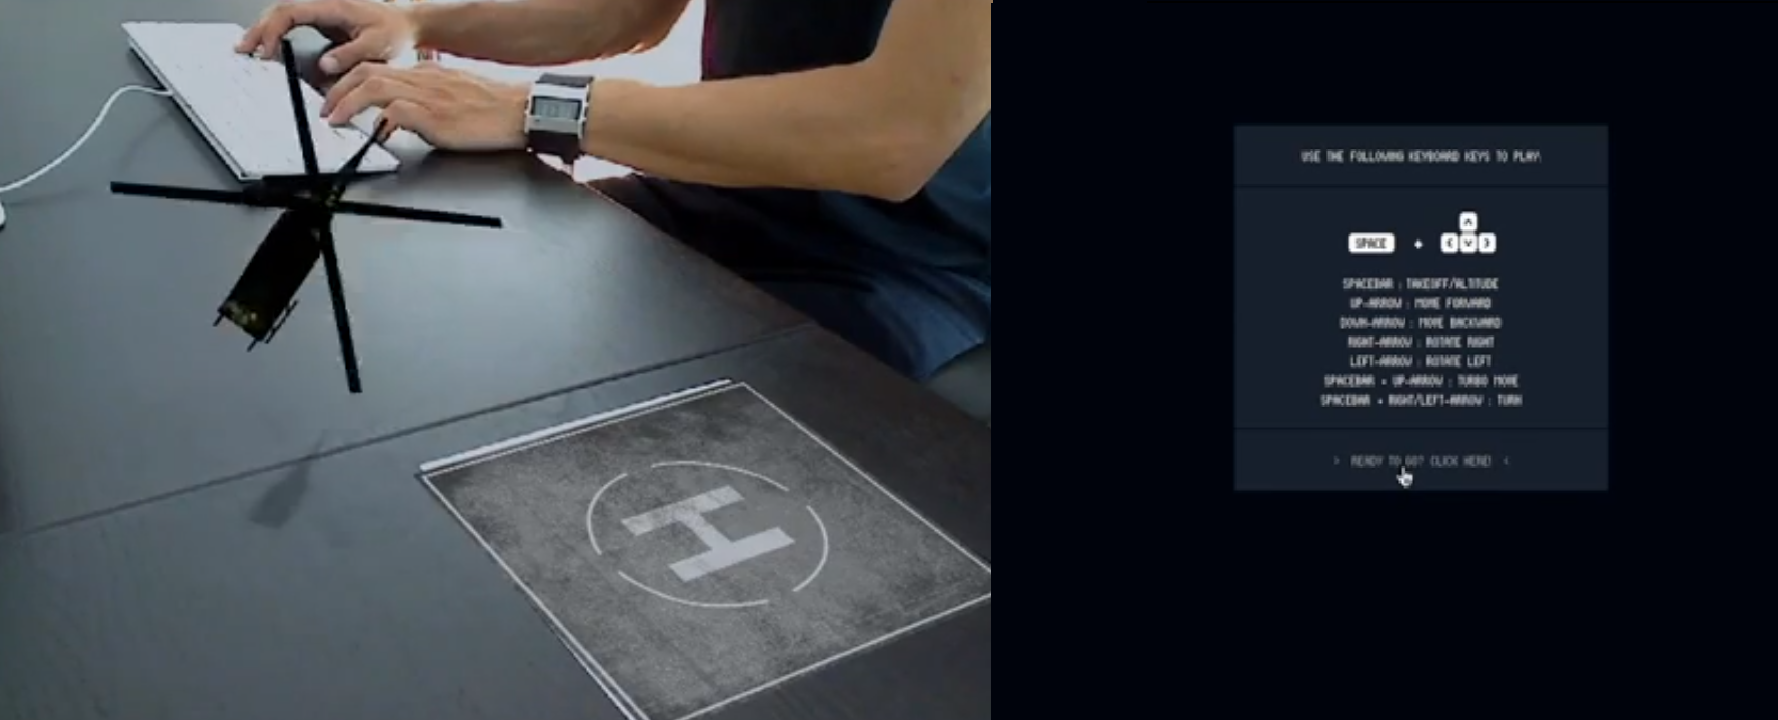
\includegraphics[width=0.95\linewidth, keepaspectratio]{helicopteroAR}
  \caption{Aplicación que permite controlar un helicóptero en realidad aumentada, a la izquierda se muestran los controles que usa para dirección y mantener vuelo}
  \label{fig:Helicoptero AR}
\end{figure}

\section{Análisis}

\subsection{Preparación del Ambiente Virtual de Desplazamiento del Drone}
Como sabemos cuando hablamos de Realidad Aumentada, los entornos en donde se efectúa esto, en la gran mayoría de los casos, se incluye una imágen o patrón fiduciario el cual nos ayuda a renderizar modelo 3D. Estas patrones fiduciales, son imágenes que se colocan sobre superficies físicas y las cuales nos ayudan a conocer sobre su alineación, idenficación y seguimiento ~\cite{bestfiducial}. Estos Patrones nos ayudan a conocer una posición relativa entre el Patrón y nuestro Modelo Aumentado en 3D. Es por eso que nos inclinaremos al uso de estos Patrones Fiduciales en la preparación inicial del ambiente virtual, ya que es perfecto para referenciar el punto inicial de movimiento de nuestro Drone en 3D en un entorno Aumentado.

Para simular colisiones con el Ambiente Real, se propone usar las Cámaras Infrarrojas para hacer un reconocimientos de las paredes del Ambiente, y así poder representar límites en el ambiente Virtual.

\subsection{Modelo 3D de Nuestro Drone}
En otros proyectos observamos que se usan helicópteros o quadrocopters para proyectos de RA. Ahora en el nuestro usaremos otro modelo, el cual fue de nuestro agrado. El Drone que utilizaremos para este Proyecto, es el modelo de un Drone militar Predator. El Drone Predator es uno de los aviones no Tripulados más usados en misiones de reconocimiento, inteligencia, bombardeo, y más. Este avión militar es No Tripulado, y lo maneja un experto asignado desde un centro de comando militar. 


\begin{figure}[h!]
  \centering
  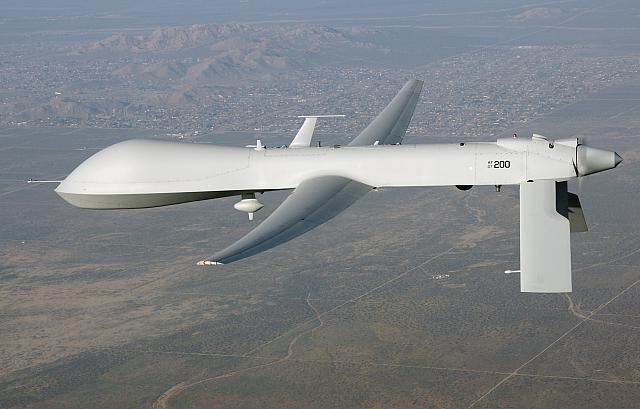
\includegraphics[width=0.95\linewidth, keepaspectratio]{predator}
  \caption{Drone Predator es uno de los aviones Militares No tripulado más usados en misiones de Reconocimiento e Inteligencia. Brinda Soporte a la Armada y Marina de los Estados Unidos.}
  \label{fig:Drone Predator}
\end{figure}

Debido a que este Avión es a Control Remoto, es perfectamente acorde a lo que queremos desarrollar en nuestro Proyecto. \\
La diferencia que hay entre Helicopteros y nuestro Drone Predator, es que un Helicoptero puede mantenerse quieto en un lugar, mientras que el Drone mantendrá siempre un movimiento hacia delante desde su propio eje mientras este en vuelo. Ahora debemos recrear esto en un entorno de RA.

\subsection{Determinación de Perspectiva Durante el Movimiento de Dispositivo Mediante GPS}
Una vez detectado el patrón fidusial del Drone y finalizado su renderizado, el seguimiento del Drone pasa a ser por GPS tomando como referencias la posición dada por el GPS del dispositivo y el \textit{offset} de el punto virtual del patrón fidusial, luego de esto se puede hacer seguimiento del modelado sin necesidad de apuntar al patrón fidusial.

%\subsection{Captura del Entorno Para Simulación de la Visión del Drone}

\subsection{Control del Drone}
Debido a que utilizaremos OpenGL para el modelado 3D de nuestro Drone. Para el control del mismo podríamos utilizar esta misma herramienta para determinar movimiento y posición en el ambiente virtual. OpenGL incluye métodos para poder transformar o mover modelos 3D respecto a un eje que nosotros podemos definir. Entonces se puede usar esta metodología de movimiento sobre un eje determinado, convirtiendo a nuestro patrón fiducial en el origen de este eje por el cual nuestro Drone en 3D interactuará, este patrón fidusial haría las veces de \textit{helipuerto} sobre el cual el Drone es renderizado y despega.\\
Para controlar diferentes comportamientos de nuestro Drone 3D, tal como Subir, Bajar, Acelerar o Detenerse; usaremos un Control de eventos que se lanzan al momento en que el ususario interactúa con la interfaz de usuario de la aplicación, y gracias a estos eventos podríamos brindarle comportamientos diferentes a nuestro Drone.\\
Esta interfaz de usuario constaría con 2 joystick que permitirían rotar y desplazar el Drone sobre la vista de cámara con la que se podrá realizar el seguimiento del Drone. También teníamos pensando añadirle un botón de disparo de un misil, pero esto sería algo mas para mejorar la estética por ahora.

\section{Recursos}
\begin{enumerate}
  \item Tablet Android con soporte para gráficos 3D
  \item WorkStation
  \item Herramientas de Desarrollo para Android
  \item Librerías OpenGL, ARToolkit for Android
\end{enumerate}

%content

%\subsection{A subsection}

%More text before content table.

%%%BIBLIOGRAPHY
%\bibliographystyle{abbrv}
\bibliographystyle{plainnat}
\bibliography{PropuestaProyecto}  % PropuestaProyecto.bib is the name of the Bibliography in this case
\end{document}
